\documentclass[border=10pt]{standalone}
\usepackage{tikz}
\usepackage[svgnames]{xcolor}
\usepackage{amsmath,amsfonts,amssymb}
\usetikzlibrary{positioning, calc, fit, arrows.meta, backgrounds, shapes.geometric}

\begin{document}
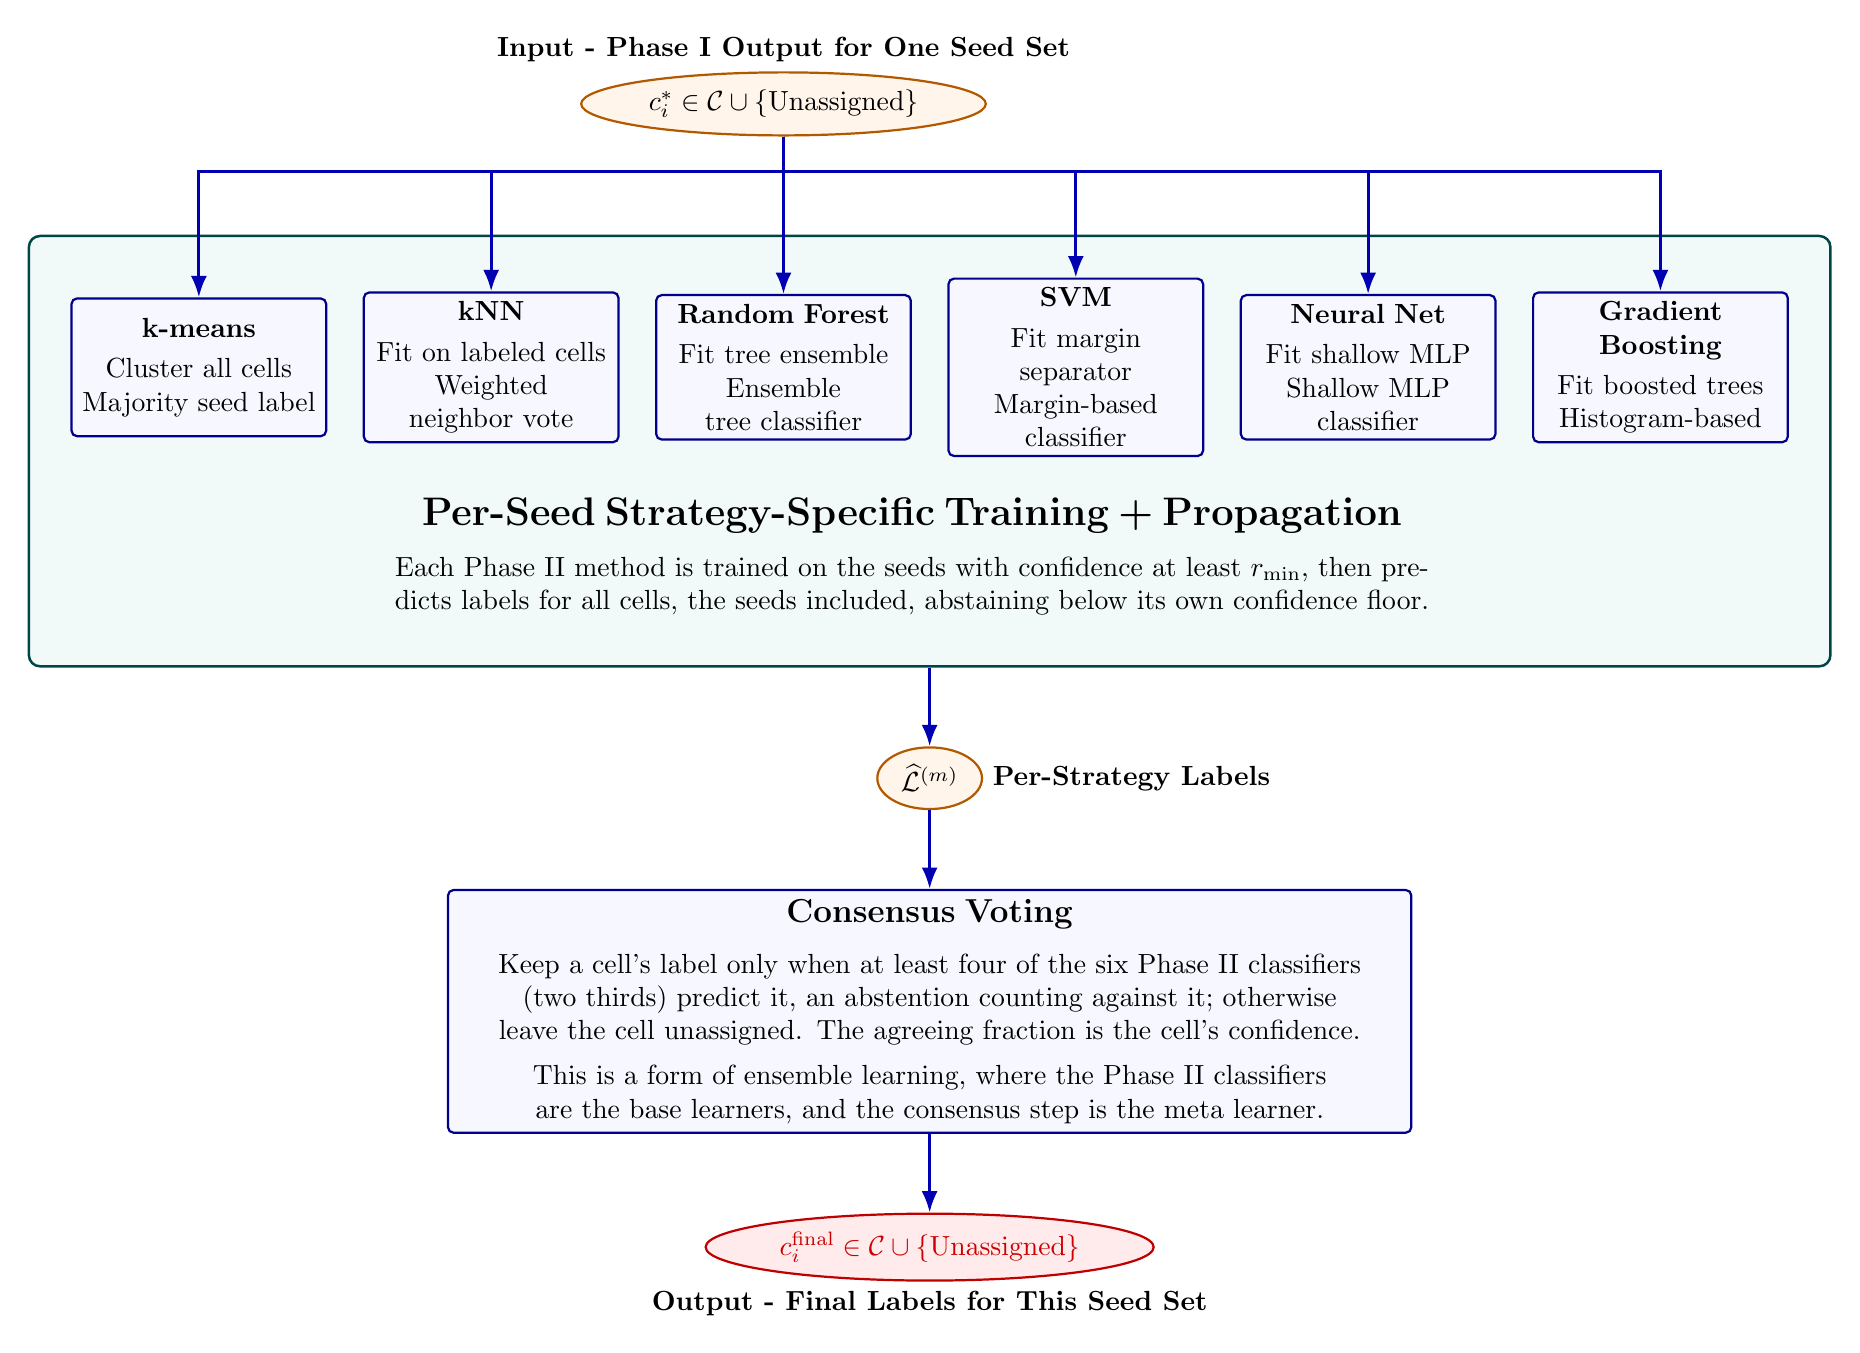
\begin{tikzpicture}[
    >=Latex,
    box/.style={draw=blue!55!black, line width=0.8pt, rectangle, align=center, minimum height=1.2cm, minimum width=2.5cm, fill=blue!3, rounded corners=2pt},
    container/.style={draw=teal!55!black, line width=0.9pt, rectangle, inner sep=15pt, align=center, rounded corners=4pt, fill=teal!5},
    var/.style={draw=orange!70!black, line width=0.8pt, ellipse, align=center, inner sep=3pt, fill=orange!8},
    flow/.style={->, line width=1.05pt, draw=blue!70!black},
    bypass/.style={->, dashed, line width=1.0pt, draw=red!70!black},
    txt/.style={align=center, font=\Large\bfseries}
  ]

  
  \node[var, label=above:\textbf{Input - Phase I Output for One Seed Set}] (input) {$c_i^* \in \mathcal{C} \cup \{\text{Unassigned}\}$};

  
  \node[box, below=2.0cm of input, text width=3.0cm, minimum height=1.75cm] (rf) {
    {\bfseries Random Forest}\\[0.6ex]
    Fit tree ensemble\\
    Ensemble tree classifier
  };
  \node[box, left=0.45cm of rf, text width=3.0cm, minimum height=1.75cm] (knn) {
    {\bfseries kNN}\\[0.6ex]
    Fit on labeled cells\\
    Weighted neighbor vote
  };
  \node[box, left=0.45cm of knn, text width=3.0cm, minimum height=1.75cm] (centroid) {
    {\bfseries k-means}\\[0.6ex]
    Cluster all cells\\
    Majority seed label
  };
  \node[box, right=0.45cm of rf, text width=3.0cm, minimum height=1.75cm] (svm) {
    {\bfseries SVM}\\[0.6ex]
    Fit margin separator\\
    Margin-based classifier
  };
  \node[box, right=0.45cm of svm, text width=3.0cm, minimum height=1.75cm] (nn) {
    {\bfseries Neural Net}\\[0.6ex]
    Fit shallow MLP\\
    Shallow MLP classifier
  };
  \node[box, right=0.45cm of nn, text width=3.0cm, minimum height=1.75cm] (hgb) {
    {\bfseries Gradient Boosting}\\[0.6ex]
    Fit boosted trees\\
    Histogram-based
  };

  \node[below=0.6cm of rf.south east, text width=20.0cm, align=center] (prop_label) {
    {\Large\bfseries Per-Seed Strategy-Specific Training + Propagation}\\[1.5ex]
    Each Phase II method is trained on the seeds with confidence at least $r_{\min}$, then predicts labels for all cells, the seeds included, abstaining below its own confidence floor.
  };

  
  \begin{scope}[on background layer]
    \node[container, fit=(knn) (centroid) (rf) (svm) (nn) (hgb) (prop_label)] (propagation) {};
  \end{scope}

  
  \node[var, below=1.0cm of propagation, label=right:\textbf{Per-Strategy Labels}] (preds) {$\widehat{\mathcal{L}}^{(m)}$};

  
  \node[box, below=1.0cm of preds, text width=12cm, minimum height=3.0cm] (consensus) {
    {\large\bfseries Consensus Voting}\\[1.5ex]
    Keep a cell's label only when at least four of the six Phase II classifiers (two thirds) predict it, an abstention counting against it; otherwise leave the cell unassigned. The agreeing fraction is the cell's confidence.\\[1ex]
    This is a form of ensemble learning, where the Phase II classifiers are the base learners, and the consensus step is the meta learner.
  };

  
  \node[var, below=1.0cm of consensus, text=red!80!black, fill=red!8, draw=red!75!black, label=below:\textbf{Output - Final Labels for This Seed Set}] (output) {$c_i^{\mathrm{final}} \in \mathcal{C} \cup \{\text{Unassigned}\}$};

  
  \draw[flow] (input.south) -- ++(0,-0.45) -| (knn.north);
  \draw[flow] (input.south) -- ++(0,-0.45) -| (centroid.north);
  \draw[flow] (input.south) -- ++(0,-0.45) -| (rf.north);
  \draw[flow] (input.south) -- ++(0,-0.45) -| (svm.north);
  \draw[flow] (input.south) -- ++(0,-0.45) -| (nn.north);
  \draw[flow] (input.south) -- ++(0,-0.45) -| (hgb.north);
  \draw[flow] (propagation.south) -- (preds.north);
  \draw[flow] (preds.south) -- (consensus.north);
  \draw[flow] (consensus.south) -- (output.north);

\end{tikzpicture}
\end{document}
